\section{Experiments}
\label{sec:experiments}

\subsection{Setup}
For each backbone and each fold we fine-tune one model per training degradation: \emph{bicubic}, \emph{generic}, \emph{bicubic + JPEG 75} and \emph{measured}. All use the recipe of Section~\ref{sec:stable} and differ in nothing else, so differences between them are attributable to the degradation. Together with the two ablation runs per fold of Table~\ref{tab:stability} and the two JPEG-only variants of Section~\ref{sec:ablation} this gives \NRuns{} runs over the \NFolds{} folds. Models are compared with bicubic interpolation and with the published weights of the same backbone on four cells: AMI with 36-pixel inputs (\NAmiImg{} images of \NAmiSubj{} subjects), EarVN1.0 with 24-pixel inputs (\NEarvnImg{} images, \NEarvnSubj{} subjects) and AWEx with 24 and 36-pixel inputs (\NAwexSImg{} and \NAwexMImg{} images).

\subsection{The training degradation decides}
Table~\ref{tab:matrix} crosses the training degradation with the degradation of the test input, for SPAN on AMI. Three observations follow. First, fine-tuning on ear images with bicubic downsampling improves the clean column and nothing else: under compression the fine-tuned model is as far below bicubic interpolation as the published weights. Domain data without the right degradation does not help. Second, the generic pipeline yields a model that is below bicubic interpolation on clean inputs on all four cells (by \GenVsBicCleanMin{} to \GenVsBicCleanMax{}~dB) and between \GenVsBicEstMin{} and \GenVsBicEstMax{}~dB of it on inputs degraded with the measured pipeline; it is the best choice only on inputs produced by the generic pipeline itself, which the classifier of Section~\ref{sec:measured} shows to be unlike real small ear images. Third, on JPEG~75 inputs the measured degradation recovers \DegEffMin{} to \DegEffMax{}~dB over bicubic training across the four cells, and the fixed JPEG~75 degradation \JpgEffMin{} to \JpgEffMax{}~dB. This is an order of magnitude more than the \SpreadQLow{}~dB that separates the \NPub{} published architectures under the same inputs (Section~\ref{sec:capacity}).

\begin{table}[t]
\centering
\caption{PSNR-Y (dB) of SPAN on AMI (36-pixel inputs) by training degradation (rows) and test input (columns). Best fine-tuned or published model per column in bold.}
\label{tab:matrix}
\resizebox{\linewidth}{!}{%
\begin{tabular}{@{}lccccc@{}}
\toprule
 & \multicolumn{5}{c}{Test input} \\
\cmidrule(l){2-6}
Training degradation & Clean & JPEG 93 & JPEG 75 & Measured & Generic \\
\midrule
\tabinput{generated/tab_matrix}
\bottomrule
\end{tabular}}
\end{table}

\subsection{Main result}
Table~\ref{tab:main} gives the paired differences between SPAN fine-tuned with the measured degradation and each reference, on inputs degraded with the measured pipeline. The model exceeds bicubic interpolation by \EstVsBicMin{} to \EstVsBicMax{}~dB, the published weights by \EstVsPubMin{} to \EstVsPubMax{}~dB and the generic pipeline by \EstVsGenMin{} to \EstVsGenMax{}~dB; no confidence interval contains zero. LPIPS improves as well, by \EstLpipsVsBicMin{} to \EstLpipsVsBicMax{} over bicubic interpolation and by \EstLpipsVsGenMin{} to \EstLpipsVsGenMax{} over the generic pipeline. The result holds in each fold separately, including the two held-out folds (measured minus generic on AMI: \EstVsGenFoldMin{} to \EstVsGenFoldMax{}~dB across folds), on inputs compressed at a single quality (\EstVsBicQLowMin{} to \EstVsBicQLowMax{}~dB over bicubic at quality 75 and \EstVsBicQHighMin{} to \EstVsBicQHighMax{}~dB at quality 93), and for the second backbone: DISP fine-tuned with the measured degradation exceeds bicubic interpolation by \DispEstVsBicMin{} to \DispEstVsBicMax{}~dB and its generic counterpart by \DispEstVsGenMin{} to \DispEstVsGenMax{}~dB. The gain is larger for smaller inputs (Figure~\ref{fig:size}): \EstVsBicAmiS{}, \EstVsBicAmiM{} and \EstVsBicAmiL{}~dB over bicubic at 24, 36 and 48 pixels on AMI.

\begin{table}[t]
\centering
\caption{SPAN fine-tuned with the measured degradation \emph{minus} each reference, on inputs degraded with the measured pipeline. Paired differences with 95\% confidence intervals (bootstrap over subjects).}
\label{tab:main}
\resizebox{\linewidth}{!}{%
\begin{tabular}{@{}lcccc@{}}
\toprule
Ours minus & AMI, 36 px & EarVN1.0, 24 px & AWEx, 24 px & AWEx, 36 px \\
\midrule
\tabinput{generated/tab_main}
\bottomrule
\end{tabular}}
\end{table}

\begin{figure}[t]
\centering
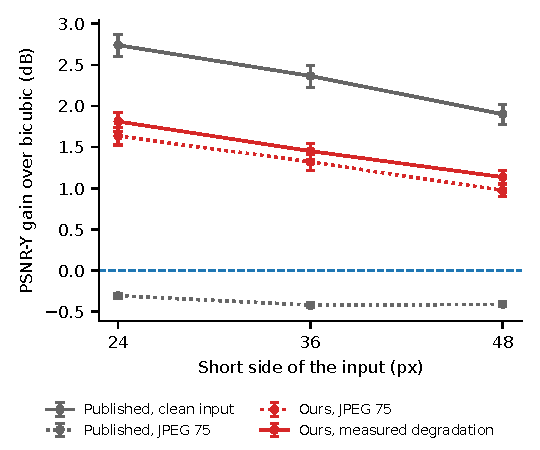
\includegraphics[width=0.55\linewidth]{figures/fig_size.pdf}
\caption{PSNR gain over bicubic interpolation by input size on AMI, for the published SPAN weights and for SPAN fine-tuned with the measured degradation. Bars: 95\% confidence intervals.}
\label{fig:size}
\end{figure}

\paragraph{The price} The model is specialised to compressed inputs. On clean inputs it is \EstVsPubCleanMin{} to \EstVsPubCleanMax{}~dB below the published weights, while remaining above bicubic interpolation (Table~\ref{tab:matrix}). No single model is best for every input. Since real small ear images are compressed, we regard the trade as the right one for this domain, and report the clean column so that the reader can judge.

\subsection{What part of the measured degradation matters?}
\label{sec:ablation}
The realism classifier could not distinguish the measured degradation from bicubic downsampling followed by JPEG at quality 75. Table~\ref{tab:levels} asks the same question of the trained models. Against a model trained with the fixed quality 75, the measured degradation is better by \EstVsJpgHighMin{} to \EstVsJpgHighMax{}~dB on quality-93 inputs and by \EstVsJpgMin{} to \EstVsJpgMax{}~dB on the measured mixture, and worse by \EstVsJpgLowMin{} to \EstVsJpgLowMax{}~dB on quality-75 inputs, on which the fixed model is trained exactly. Training on the measured distribution of compression levels thus buys robustness across the levels that occur in practice for a negligible loss at any one of them.

\begin{table}[t]
\centering
\caption{Measured degradation \emph{minus} fixed JPEG~75, same backbone, by test input (PSNR-Y, dB; 95\% confidence intervals).}
\label{tab:levels}
\resizebox{\linewidth}{!}{%
\begin{tabular}{@{}llcccc@{}}
\toprule
Backbone & Test input & AMI, 36 px & EarVN1.0, 24 px & AWEx, 24 px & AWEx, 36 px \\
\midrule
\tabinput{generated/tab_levels}
\bottomrule
\end{tabular}}
\end{table}

To separate the contribution of the compression levels from that of the measured noise and blur, we train two further models: one with bicubic downsampling followed by JPEG at the measured distribution of levels, without noise or blur, and one with JPEG quality drawn uniformly from 60 to 95, which uses nothing measured from the data (Table~\ref{tab:ablation} and the corresponding rows of Table~\ref{tab:matrix}). On inputs degraded with the full measured pipeline, the measured model is ahead of the levels-only model by \EstVsMixMin{} to \EstVsMixMax{}~dB. On inputs with the same compression levels but without noise and blur the order reverses, the levels-only model being ahead by \MixVsEstOnMixMin{} to \MixVsEstOnMixMax{}~dB; it is also ahead at quality 93 (\MixVsEstHighMin{} to \MixVsEstHighMax{}~dB) and on clean inputs (\MixVsEstCleanMin{} to \MixVsEstCleanMax{}~dB). Each model is best on the inputs that match its own training, so synthesised inputs cannot decide whether the measured noise and blur are worth having. Real images can, and Section~\ref{sec:recog} finds no difference. The levels-only and the uniform-level models differ by \MixVsUniMin{} to \MixVsUniMax{}~dB on measured inputs: once the range of levels is covered, their exact distribution does not matter.

We conclude that the essential ingredient is JPEG compression over the range of quality levels found in the target images, here roughly 70 to 95. Measuring the degradation serves to identify that range; estimating noise and blur is not required. We keep the measured degradation as the reference model in all tables because it was fixed before these comparisons were run.

\begin{table}[t]
\centering
\caption{Separating compression levels from noise and blur: SPAN fine-tuned with the measured degradation \emph{minus} two JPEG-only variants (PSNR-Y, dB; 95\% confidence intervals).}
\label{tab:ablation}
\resizebox{\linewidth}{!}{%
\begin{tabular}{@{}llcccc@{}}
\toprule
Comparison & Test input & AMI, 36 px & EarVN1.0, 24 px & AWEx, 24 px & AWEx, 36 px \\
\midrule
\tabinput{generated/tab_ablation}
\bottomrule
\end{tabular}}
\end{table}

\subsection{Real small ear images: identification}
\label{sec:recog}
All results above use inputs synthesised from larger images, because real small images have no ground truth. Identity labels offer an objective measure that needs none. We take the subjects of EarVN1.0 that were used neither for SR training nor for any fitting (the test and reserved groups). For each subject, half of the large images (short side at least 96 pixels) are enrolled and their embeddings averaged into a template; \RecEnrolled{} subjects are enrolled with \RecGallery{} images. The probes are the \RecProbes{} \emph{real} small images (short side 24 to 48 pixels) of the \RecSubj{} enrolled subjects that have any. Each probe is enlarged $\times4$ by the method under test and resized to the input size of the recogniser by one fixed operation. The recogniser is a ResNet-18~\cite{he2016resnet} with a cosine-margin loss~\cite{wang2018cosface}, trained only on large images of \RecTrainSubj{} other subjects (\RecTrainImg{} images); it never sees a small or an upscaled image, so it does not favour the look of any upscaling method. As a control we repeat the experiment with frozen ImageNet features that have never seen an ear.

Table~\ref{tab:recog} reports rank-1 identification and equal error rate (EER). With large probes the recogniser reaches a rank-1 rate of \RecRankRef{}\% (EER \RecEerRef{}\%), which bounds what can be expected of small ones; on held-out images of its training subjects its accuracy is \RecValAcc{}\%. With real small probes and bicubic upscaling the rate is \RecRankBic{}\%. The methods fall into three groups.

\emph{Bicubic-trained models do not help.} The published SPAN weights reach \RecRankPub{}\% (\RecPubVsBic{} percentage points relative to bicubic upscaling), and SPAN fine-tuned on ear images with bicubic downsampling \RecRankBict{}\% (\RecBictVsBic{}).

\emph{Every compression-aware model nearly doubles the rate.} SPAN with the measured degradation reaches \RecRankEst{}\%, a paired gain of \RecEstVsBic{} points over bicubic upscaling and \RecEstVsPub{} over the published weights, and lowers the EER from \RecEerBic{}\% to \RecEerEst{}\% (\RecEerEstVsBic{}). The second backbone behaves alike (DISP: \RecRankDispEst{}\%, \RecDispEstVsBic{} over bicubic). Within the group the differences are small. The fixed JPEG~75 and uniform-level variants are indistinguishable from our model (\RecJpgVsEst{} and \RecUniVsEst{} points); the levels-only variant and the generic pipeline are about one point lower (\RecMixVsEst{} and \RecGenVsEst{}).

\emph{Large GAN-trained models are not significantly better.} BSRGAN and Real-ESRGAN reach \RecRankBsrgan{}\% and \RecRankRealesrgan{}\% (\RecBsrganVsEst{} points for BSRGAN relative to our model), at \LatRatio{} times the latency.

The control recogniser, which has never seen an ear, gives much lower rates and the same ordering: \RecCtlRankBic{}\% with bicubic upscaling, \RecCtlRankPub{}\% with the published weights and \RecCtlRankEst{}\% with our model (\RecCtlEstVsBic{} over bicubic).

\begin{table}[t]
\centering
\caption{Identification of real small ear images (short side 24 to 48 pixels) after $\times4$ upscaling. Rank-1 rate with 95\% confidence interval and equal error rate, in \%, for an ear recogniser and for frozen ImageNet features. Fine-tuned rows average the models of the folds.}
\label{tab:recog}
\resizebox{\linewidth}{!}{%
\begin{tabular}{@{}lcccc@{}}
\toprule
 & \multicolumn{2}{c}{Ear recogniser (ResNet-18)} & \multicolumn{2}{c}{ImageNet features (ResNet-50)} \\
\cmidrule(lr){2-3}\cmidrule(l){4-5}
Upscaling & Rank-1 & EER & Rank-1 & EER \\
\midrule
\tabinput{generated/tab_recog}
\bottomrule
\end{tabular}}
\end{table}

\paragraph{By compression level of the probe} The quality setting of each real probe can be read from its file, which allows a direct test of the threshold found on synthesised inputs in Section~\ref{sec:analysis}. Table~\ref{tab:recogquality} splits the probes into those stored at JPEG quality 70 to 80 (\RecQLowN{} probes of \RecQLowSubj{} subjects) and those stored at quality 90 or above (\RecQHighN{} probes of \RecQHighSubj{} subjects). For the heavily compressed probes the published SPAN weights change the rank-1 rate by \RecQLowPub{} points relative to bicubic upscaling; for the lightly compressed ones by \RecQHighPub{}. The compression-aware model gains \RecQLowEst{} and \RecQHighEst{} points. The pattern predicted from synthesised inputs, a bicubic-trained model that is useful at quality 93 and not at quality 75, is thus observed on real images through an independent measure. The table also locates the advantage of the GAN-trained models: BSRGAN gains \RecQHighBsrgan{} points on the lightly compressed probes and \RecQLowBsrgan{} on the heavily compressed ones. The two groups contain largely different subjects, so the comparison is between methods within a group, not between groups.

\begin{table}[t]
\centering
\caption{Rank-1 identification (\%) of real small ear images by the JPEG quality stored in the probe file, and paired difference from bicubic upscaling in percentage points with 95\% confidence interval (EarVN1.0, ear recogniser).}
\label{tab:recogquality}
\resizebox{\linewidth}{!}{%
\begin{tabular}{@{}lcccc@{}}
\toprule
 & \multicolumn{2}{c}{Quality 70--80} & \multicolumn{2}{c}{Quality $\geq$ 90} \\
\cmidrule(lr){2-3}\cmidrule(l){4-5}
Upscaling & Rank-1 & vs.\ bicubic & Rank-1 & vs.\ bicubic \\
\midrule
\tabinput{generated/tab_recog_quality}
\bottomrule
\end{tabular}}
\end{table}

\paragraph{A second dataset and a second recogniser} To test whether these results depend on the recogniser or on the dataset, we repeat the experiment with a second ear recogniser, a ResNet-50 trained on the same data (\RecRfValAcc{}\% accuracy on held-out images of its training subjects), and on AWEx, which was used for no training of any kind (\RecAwexEnrolled{} subjects enrolled, \RecAwexProbes{} real small probes of \RecAwexSubj{} subjects, same protocol). Table~\ref{tab:recogrobust} gives the paired differences from bicubic upscaling.

The second recogniser confirms the result on EarVN1.0: the rank-1 rate rises from \RecEarvnRfRankBic{}\% with bicubic upscaling to \RecEarvnRfRankEst{}\% with our model (\RecEarvnRfEstVsBic{} points), against \RecEarvnRfPubVsBic{} for the published weights. With this recogniser the generic pipeline is significantly below our model (\RecEarvnRfGenVsEst{} points).

AWEx behaves differently. No upscaling method changes the rank-1 rate significantly there, with either recogniser: our model by \RecAwexReEstVsBic{} and \RecAwexRfEstVsBic{} points, the published weights by \RecAwexRePubVsBic{} and \RecAwexRfPubVsBic{}, BSRGAN by \RecAwexReBsrganVsBic{} and \RecAwexRfBsrganVsBic{}. \emph{The gain observed on EarVN1.0 is not replicated on AWEx.}

\paragraph{When does upscaling help identification?} The two datasets differ in two respects, each of which bounds what an upscaling step can contribute. We examined them after seeing the AWEx result, and report them as conditions suggested by the data, not as an established explanation.

\emph{Compression.} The small AWEx images carry no JPEG block structure. The ratio of pixel differences across $8\times8$ block boundaries to differences inside blocks has a median of \BlockAwex{} for the AWEx probes, against \BlockEarvnLow{} for the EarVN1.0 probes stored at quality 70 to 80 and \BlockEarvnHigh{} for those at quality 90 or above; AWEx is distributed as PNG and its compression history is unknown. A compression-aware model has no blocking to remove there.

\emph{Headroom.} Upscaling can at best give back what low resolution took from the recogniser. We call \emph{headroom} the difference between the rank-1 rate of large probes and that of bicubically upscaled small probes. On EarVN1.0 it is large (\RecRankRef{}\% against \RecRankBic{}\% with the ResNet-18 recogniser); on AWEx, where a subject has a median of \RecAwexGalMed{} enrolled images against \RecEarvnGalMed{} on EarVN1.0, it is absent (\RecAwexReRankRef{}\% against \RecAwexReRankBic{}\%). Within EarVN1.0 the gain of our model follows the headroom of the subject: among the \HeadEarvnReSubj{} subjects with at least five small probes, the half with less headroom (\HeadEarvnReLowRoom{} points on average) gains \HeadEarvnReLowGain{} points and the half with more (\HeadEarvnReHighRoom{}) gains \HeadEarvnReHighGain{}; with the ResNet-50 recogniser the two halves gain \HeadEarvnRfLowGain{} and \HeadEarvnRfHighGain{}. The rank correlation between headroom and gain is positive but does not reach significance at this number of subjects (Spearman $\rho=\HeadEarvnReRho$, $p=\HeadEarvnReP$, and $\rho=\HeadEarvnRfRho$, $p=\HeadEarvnRfP$). Headroom alone is not sufficient: the AWEx subjects that do have it (\HeadAwexReHighRoom{} points in the upper half) gain \HeadAwexReHighGain{} and \HeadAwexRfHighGain{} points with the two recognisers, although these per-subject figures rest on a median of two probes.

In our data, then, upscaling improves identification where the probes are compressed \emph{and} the recogniser loses accuracy at low resolution. EarVN1.0 meets both conditions and AWEx neither, so the two datasets cannot separate them; the split by file quality and the split by headroom within EarVN1.0 are the only within-dataset evidence for each.

\begin{table}[t]
\centering
\caption{Robustness of the identification result: paired difference in rank-1 rate from bicubic upscaling (percentage points, 95\% confidence interval), on two datasets and with two ear recognisers. The first two rows give absolute rank-1 rates.}
\label{tab:recogrobust}
\resizebox{\linewidth}{!}{%
\begin{tabular}{@{}lcccc@{}}
\toprule
 & \multicolumn{2}{c}{EarVN1.0} & \multicolumn{2}{c}{AWEx} \\
\cmidrule(lr){2-3}\cmidrule(l){4-5}
Upscaling & ResNet-18 & ResNet-50 & ResNet-18 & ResNet-50 \\
\midrule
\tabinput{generated/tab_recog_robust}
\bottomrule
\end{tabular}}
\end{table}

Three conclusions follow. First, on real small ear images that are JPEG-compressed, the finding of Section~\ref{sec:analysis} carries over: SR trained with bicubic downsampling gives no identification benefit, with or without fine-tuning on ear data, and compression-aware training does, with two recognisers and a control. Second, the choice among compression-only degradations makes no measurable difference to identification, which settles the question left open in Section~\ref{sec:ablation}; the generic pipeline is slightly but significantly worse, in addition to its lower fidelity (Table~\ref{tab:main}). Third, the benefit is conditional: it appears where the probes are compressed and the recogniser has headroom between large and small images, it varies with the quality stored in the probe files and with the headroom of the subject, and it is absent on AWEx, where neither condition holds. We therefore do not claim that SR improves ear identification in general; we claim to have identified when it does. Figure~\ref{fig:qualitative} shows examples.


\begin{figure}[t]
\centering
\tabinput{generated/fig_qualitative}
\caption{Real small ear images from EarVN1.0 (short side 24 to 48 pixels) enlarged $\times4$. The published weights sharpen the compression blocks; the compression-aware models remove them. \todo{select examples from several subjects; check the image rights for publication.}}
\label{fig:qualitative}
\end{figure}

\subsection{Real small ear images: viewer preference}
\todo{viewer study on real small images of the reserved subjects: pairs (ours vs.\ bicubic, ours vs.\ published weights, ours vs.\ generic), number of viewers, preference rate with confidence interval. Tools: \texttt{evaluate.py --save-sr}, \texttt{viewer\_study.py}.}

\subsection{Efficiency}
\label{sec:efficiency}
The method changes the weights of the backbone and nothing else, so its cost is that of the backbone. We take real time to mean a median latency of at most 33~ms (30 frames per second) for one $48\times68$ input, the largest input size considered here. On a desktop GPU (RTX~3080, 32-bit precision) SPAN with 48 channels (\ParamsSpan{}M parameters) needs \LatSpan{}~ms and DISP \LatDisp{}~ms, against \LatBsrgan{}~ms for BSRGAN (Table~\ref{tab:published}).

To test the claim on consumer hardware we convert the models to Core ML with 16-bit weights and measure them on an \PhoneName{} (\PhoneChip{}, iOS \PhoneOs{}), a phone released in 2020, with the performance tool of Xcode, which reports the median prediction time on the device. Table~\ref{tab:latencyios} gives the result with computation restricted to the CPU and with all compute units (CPU, GPU and neural engine) allowed. SPAN runs in \LatPhoneSpanCpu{}~ms on the CPU alone and \LatPhoneSpanAll{}~ms with all units; DISP in \LatPhoneDispCpu{} and \LatPhoneDispAll{}~ms; BSRGAN in \LatPhoneBsrganCpu{} and \LatPhoneBsrganAll{}~ms. \todo{state which models meet the 33~ms threshold once the measurements exist; if SPAN does not, change ``Real-Time'' in the title. The tool reports medians only; no 95th percentile is available.} The converted models reproduce the PyTorch outputs to within 16-bit rounding (PSNR between the two outputs: \CoremlPsnrSpan{}~dB for SPAN and \CoremlPsnrDisp{}~dB for DISP).

\begin{table}[t]
\centering
\caption{Median latency (ms) for one $48\times68$ input at $\times4$: desktop GPU (RTX~3080, PyTorch, 32-bit) and smartphone (\PhoneName{}, Core ML, 16-bit).}
\label{tab:latencyios}
\small
\begin{tabular}{@{}lrccc@{}}
\toprule
 & Params & Desktop & \multicolumn{2}{c}{Smartphone} \\
\cmidrule(l){4-5}
Model & (K) & GPU & CPU only & All units \\
\midrule
\tabinput{generated/tab_latency_ios}
\bottomrule
\end{tabular}
\end{table}
